\chapter{Etude conceptuelle}
\markboth{Chapitre 3. Etude conceptuelle}{} 
\begin{spacing}{1.2}
\minitoc
\thispagestyle{MyStyle}
\end{spacing}
\newpage

\section*{Introduction}
Le chapitre suivant marque une étape cruciale dans le processus de développement de notre plateforme de bibliothèque numérique. Cette phase englobe plusieurs aspects essentiels, notamment l'étude de l'existant, la définition précise des fonctionnalités attendues et la création d'un dictionnaire des données pour structurer les informations manipulées par la plateforme et les diagrammes de classe.\par
Dans ce chapitre, nous explorerons en détail chacun de ces éléments, en mettant en lumière leur importance dans la conception de notre plateforme.\par

Dans l'ensemble, ce chapitre constitue une étape fondamentale dans le processus de développement de notre plateforme de bibliothèque numérique. En explorant l'existant, la définition des fonctionnalités la création du dictionnaire des données et la mise en place des diagrammes de classe, nous jetterons les bases d'une conception solide et fonctionnelle, garantissant ainsi le succès de notre projet.
\par
\section{Etude de l'existant}
L'étude de l'existant permet au développeur de s'imprégner du fonctionnement et de recueillir les informations nécessaire du système actuel (ancien système) pour avoir une vision du futur système(système à concevoir).\par
Dans notre cas, l'étude de l'existant nous a permis de de faire ressortir les fonctionnalités qui seront greffé à notre bibliothèque ainsi que les information nécessaire à sa mise en place et son bon fonctionnement.

\subsection{Définition des Fonctionnalités }
La définition des fonctionnalités de notre plateforme de bibliothèque numérique constitue une étape importante dans notre processus de développement. Ces fonctionnalités sont conçues pour répondre aux attentes et pour offrir une expérience utilisateur fluide et efficace. Parmi les fonctionnalités clés que nous avons identifiées, nous pouvons citer :

a) Mise en ligne de document : Les utilisateurs ont la possibilité de mettre en ligne leurs documents, tels que des thèses, des mémoires ou des articles de recherche, sur la plateforme. Cette fonctionnalité intuitive et conviviale permet aux auteurs de partager leurs travaux avec la communauté académique de manière simple et efficace.\par


b) Validation de la mise en ligne : Avant la publication définitive sur la plateforme, les documents soumis font l'objet d'une validation par un administrateur désigné. Cette étape de validation garantit la qualité et la pertinence des documents publiés, tout en assurant le respect des normes et éthiques.\par

c) Recherche de document avec mots-clés : Les utilisateurs peuvent effectuer des recherches avancées sur la plateforme en utilisant des mots-clés spécifiques. Cette fonctionnalité permet une exploration efficace de la base de données, en permettant aux utilisateurs de trouver rapidement des documents pertinents dans leur domaine d'intérêt.\par

d) Publication de préoccupations : Les utilisateurs ont la possibilité de publier des préoccupations ou des questions relatives aux documents disponibles sur la plateforme. Cette fonctionnalité encourage l'interaction et la collaboration entre les membres de la communauté académique, en permettant aux utilisateurs de partager leurs réflexions et leurs interrogations avec leurs pairs.

\subsection{Dictionnaire des données}
Le dictionnaire des données constitue la pierre angulaire de la structure de notre plateforme de bibliothèque numérique. Il offre une vue exhaustive et des attributs qui composent notre système ainsi que leurs description et typage. Le dictionnaire de données nous fournira  un cadre solide pour la gestion et l'exploitation des données.\par
Les attributs dont nous avons fait usage  consignés dans le tableau ci-dessous.
\par 

 
\begin{table}[h!]
    \centering
    \begin{tabular}{|p{4cm}|p{5cm}|p{4cm}|}
        \hline
      \textbf{Attribut}   & \textbf{Description} & 		   \textbf{Type de données}  \\
      \hline
       id & indentifiant des entités & entier \\
        \hline
  
   nom & nom des utilisateurs & chaine de caractère \\
      \hline
     
 prenom & prenom des utilisateurs & chaine de caractère \\
   \hline
         email & email des utilisateurs & chaine de caractère \\
        \hline
        password & mot de passe pour certains utilisateurs & chaine de caractère \\
   \hline
              matricule & matricule des utilisateurs & chaine de caractère \\
        \hline
         ressource\_id & identifiant des ressources & entier  \\
        \hline
         sujet & Description de la préoccupation & texte 
 \\
        \hline
         preocupation & préoccupation des utilisateurs & texte 
 \\        
        \hline
         user\_id & id des utilisateurs dans d'autres entités & Chaine de caractère \\
        \hline
         ufr\_id & identifiant des UFR & entier \\
        \hline
         theme & thème des travaux & texte \\
        \hline
         image & photo de la page de garde & chaine de caractère \\
        \hline
         document & nom du document & chaine de caractère \\
        \hline
         date & date de soutenance & chaine de caractère \\
        \hline
         ref & identifiant de la nature d'un commentaire & entier \\
        \hline
         contenu & contenu de commentaire & texte \\
        \hline
       
     
    \end{tabular}
    \caption{Dictionnaire des données}
    \label{Tableau:Dictionnaire des données}
\end{table}


\section{Diagrammes UML}
Les diagrammes de classes UML permettent de modéliser, de manière déclarative, la structure statique d'un domaine applicatif, en termes de concepts et de relations entre eux \cite{berardi2005reasoning}. 
Dans cette section, nous présenterons les différents diagrammes qui nous on servi dans l'élaboration de notre plateforme. 

\subsection{Diagrammes de classe}
Les diagrammes de classe ont fait partie intégrante de la modélisation orientée objet et ont permis de visualiser la structure statique du système en définissant les classes, leurs attributs, leurs méthodes ainsi que les relations entre elles.\par

Ces diagrammes nous ont offert une représentation claire et structurée de notre système, facilitant ainsi la compréhension des différentes composantes et de leurs interactions. En établissant un modèle précis, nous avons pu identifier les éléments clés et leurs connexions, ce qui a aidé à garantir la cohérence et la robustesse de l'architecture de notre application.\par

Dans cette section, nous détaillons les différents diagrammes de classe élaborés pour notre projet.\par

	\begin{figure}[H]%
    \center%
    \setlength{\fboxsep}{5pt}%
    \setlength{\fboxrule}{0.5pt}%
    \fbox{
    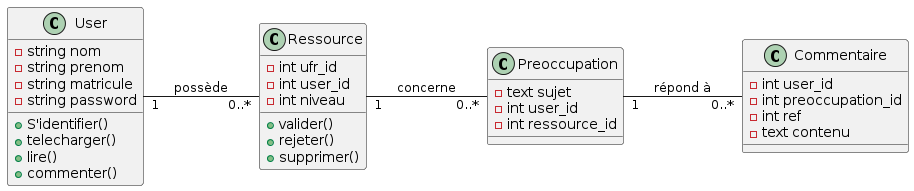
\includegraphics[width=16cm,height=4.7cm]{images/diagramme de classes.png}%
    }
    \caption{Diagrammes des classe}%
\end{figure} \par
\subsection{Diagrammes de séquence}

\textbf{Séquence :} Envoi de document sur la plateforme.
Ce diagramme de séquence montre comment se déroule le processus d'envoi de document sur la plateforme.
\begin{figure}[H]%
    \center%
    \setlength{\fboxsep}{5pt}%
    \setlength{\fboxrule}{0.5pt}%
    \fbox{
    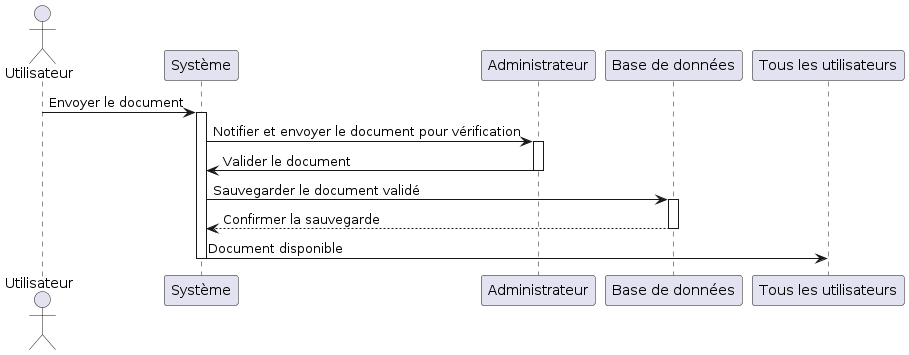
\includegraphics[width=12.5cm,height=6cm]{images/uml envoi doc.png}%
    }
    \caption{Séquences d'envoi de document}%
\end{figure}
\par
\textbf{Séquence : Envoi de préoccupation}
Ce diagramme de séquence montre comment se déroule le processus d'un envoi de préoccupation par un utilisateur à un auteur de document sur la plateforme.

\begin{figure}[H]%
    \center%
    \setlength{\fboxsep}{5pt}%
    \setlength{\fboxrule}{0.5pt}%
    \fbox{
    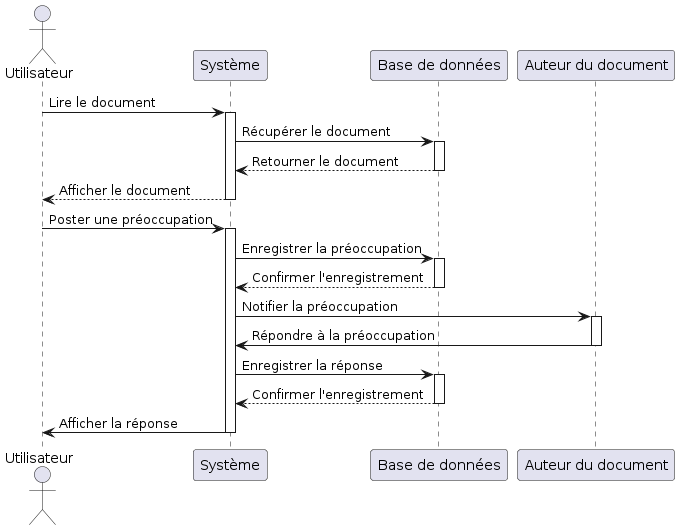
\includegraphics[width=12.5cm,height=9cm]{images/sequence preocupation.png}%
    }
    \caption{Séquences d'envoi de préoccupation}%
\end{figure}

\subsection{Règles de gestion}
Pour atteindre nos objectifs nous avons intégré dans notre système un certain nombre de règle pour un bon traitement des information. Ces règles sont les suivantes:
\renewcommand{\labelitemi}{\tiny$\bullet$}
\begin{itemize}[leftmargin=2cm, topsep=0pt]
        \begin{spacing}{1.25}
        
        \item Chaque UFR regroupe un ensemble de document.
        \item Chaque document est associé à un auteur.
        \item Chaque préoccupation est associée à un document spécifique.
        \item Chaque réponse est associée à une préoccupation correspondante.
        \end{spacing}
\end{itemize}
\begin{spacing}{0.5}
\end{spacing}

\section*{Conclusion}
L'étude conceptuelle nous a permis de voir sur papier comment sera conçu notre plateforme ainsi que les rouage nécessaires à son bon fonctionnement. Une fois établis nous avons eu à notre disposition une feuille de route bien solide pour entamer l'étape de la concrétisation.